\chapter{Integrating categorical and continuous aspects of pitch accents}
\label{chapter_onglide_modelling}

The first analysis of the controlled corpus of prosodic focus marking is concerned with intonation contours, more specifically with nuclear pitch accents. The results outlined in this chapter show that parameters of pitch accents are used in a categorical as well as a continuous manner at the same time. The two kinds of using F0 modulations seem to be applied by speakers to achieve the same -- or at least comparable -- communicative ends. This striking parallel is implemented in a first sketch of a dynamical model. The model conceptualises pitch accents as attractors in a continuous phase space. In doing so, it is able to capture the categorical nature of pitch accents, continuous variation within one pitch accent category and the generalisation that the categorical and the continuous use of intonation are related. In addition, two subgroups of speakers are identified that exhibit different patterns of intonational focus marking. Despite their differences, the behaviour of both groups can be described by means of the same model.

\section{Results of F0 measures}

As outlined in Chapter \ref{chapter_data}, the nuclear pitch accents in the corpus are assessed using two continuous parameters: tonal onglide and alignment of the peak. This section outlines the results of the two measures. Since the present chapter deals with nuclear accents only, the background condition is not included in the analyses since the vast majority (99\%) of target words in the background condition were unaccented. A treatment of this condition is added to the analysis in the next chapter (Chapter \ref{chapter_multi_prosody}).

\subsection{Tonal onglide}

Before turning to the results of the tonal onglide, it is useful to consider some example contours from the corpus. Gaining an impressionistic perspective of the data is particularly helpful in discussing tonal onglide since this measure is far less established in the research literature than the alignment of the peak. Figure \ref{fig:example_contours} presents one instance of broad (top), narrow (middle) and contrastive focus (bottom) each produced by male speaker. The stressed syllable of the target word is marked by the blue box, the arrows illustrate the F0 movement that is captured by the tonal onglide measure. The informative value of these examples is of course limited since they only represent individual utterances. However, accompanying the quantitative results, they help to give a thorough insight into the data. The figure shows that the speaker uses a falling accent in broad focus and rising accents in narrow focus and contrastive focus. Comparing these last two conditions, a larger magnitude of the rise can be attested in contrastive focus. As the following quantitative results show, this first impression is supported by the data set but there is more variation involved. \largerpage{}

\begin{figure}[b]
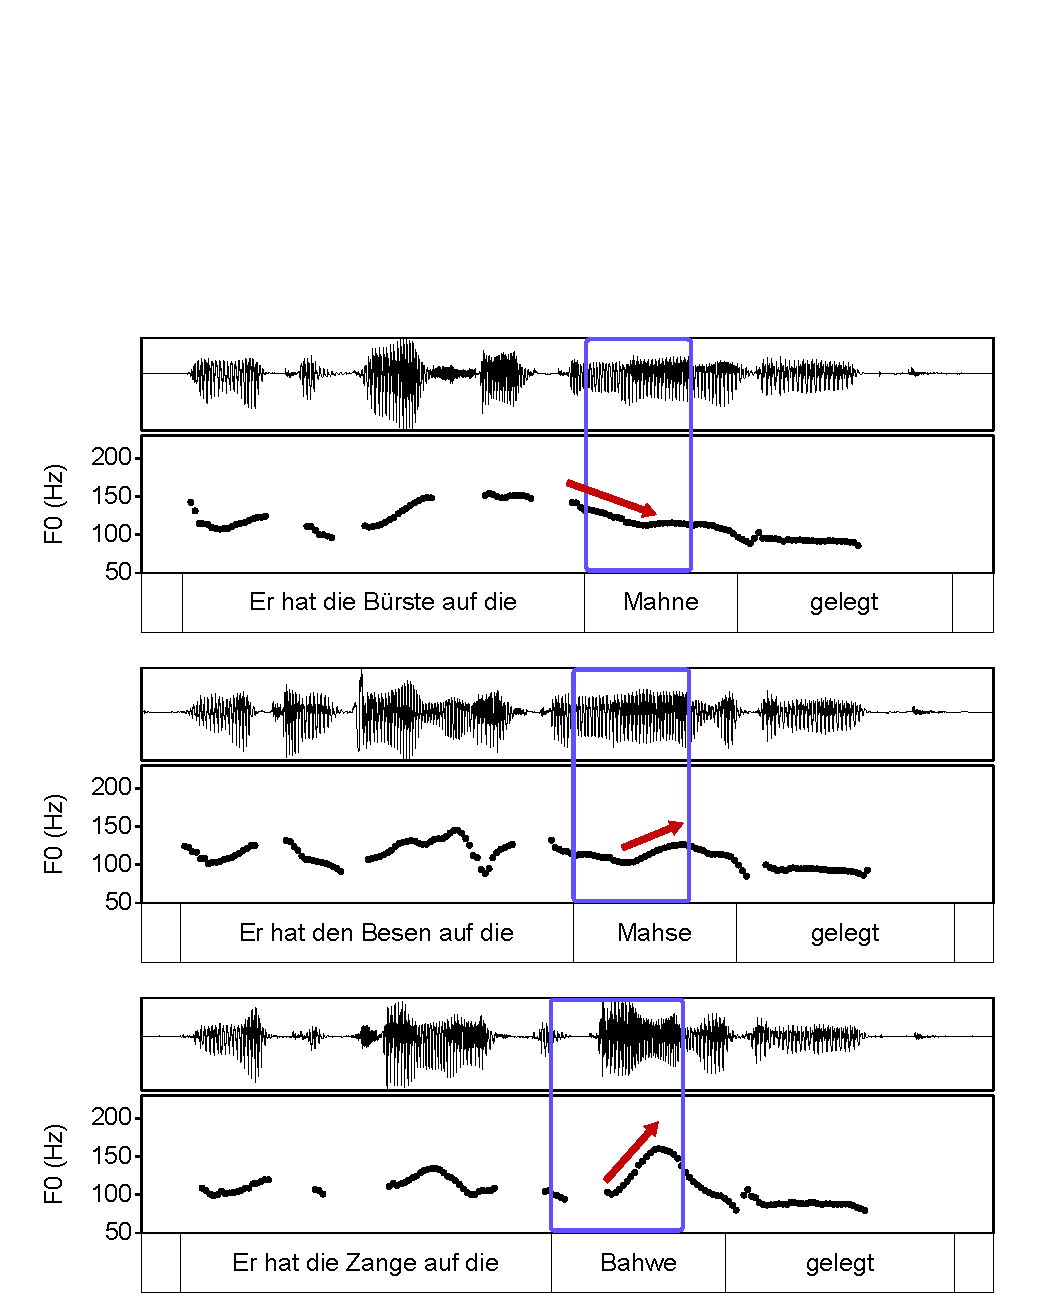
\includegraphics[width=.95\textwidth]{figures/ch6/intonation_contours.pdf}
\caption[Examples of intonation contours for broad, narrow, and contrastive focus.]{Example intonation contours for broad (top), narrow (middle), and contrastive focus (bottom). The blue box marks the nuclear accented syllable. The red arrows indicate the direction of the tonal onglide.}
\label{fig:example_contours}
\end{figure}

Figure \ref{fig:onglide_distributions_within} plots the distributions of normalised onglide values of all speakers together for broad focus, narrow focus and contrastive focus. Note that negative onglides indicate a falling tonal movement while positive onglides indicate a rising tonal movement. Broad focus is characterised by an almost symmetrical bimodal distribution, reflecting the fact that both falling and rising accents are equally possible in this focus condition. Moving on to narrow focus, the right mode of the distribution grows, indicating that the majority of accents are rising in this condition. This trend is continued in contrastive focus for which an even higher proportion of rising accents is found. The numbers and proportions of falling and rising onglides are summarised in Table \ref{tab:props_onglide}. In a minority of cases (6 cases, 0.38\% of the data), it was not possible to track the F0 at the locations marked by the labellers, rendering the onglide measure impossible to apply (labelled ``NA" in the table).

\begin{figure}[!h]
	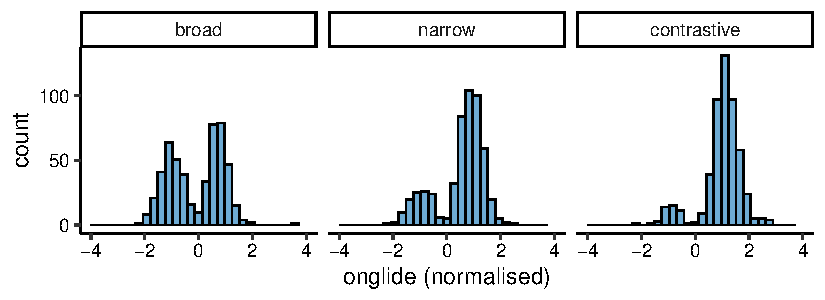
\includegraphics[width=.95\textwidth]{figures/ch6/onglide_norm_distribution_within.pdf}
	\caption{Distributions of normalised tonal onglide values for broad, narrow and contrastive focus.}
	\label{fig:onglide_distributions_within}
\end{figure}

\begin{table}[!h]
	\caption{Proportions of falling and rising onglides.}
	\begin{tabularx}{\textwidth}{Xllll}
		\lsptoprule
		\textbf{focus types	} &	\textbf{falling accents}&		\textbf{rising accents} &			\textbf{NA} & 	\textbf{all}\\
		&				\textbf{(negative onglides)} &	\textbf{(positive onglides)} &		&			\\	
		\midrule
		broad focus &		241 (47.07\%) & 				270 (52.73\%)  & 					1 (0.2\%) &			512 \\
		%&				47.07\% &				52.73\% &					0.2\% &		\\
		\midrule
		narrow focus &		115 (21.78\%)  &				411 (77.84\%) & 					2 (0.38\%)  &			528 \\
		%&				21.78\% &				77.84\% & 					0.38\% &		\\
		\midrule
		contrastive focus &		47 (9.04\%)  &					470 (90.38\%) &						3 (0.58\%) &			520 \\
		%&				9.04\% &				90.38\% &					0.58\% &		\\
		\midrule
		all &				403 (25.83\%) &					1151 (73.78\%)  &					6 (0.38\%) &			1560\\\lspbottomrule
		%&				25.83\% & 				73.78\% &					0.38\% & 		\\ \lspbottomrule\lspbottomrule
	\end{tabularx}
	\label{tab:props_onglide}
\end{table}
The distributions reveal that there is no one-to-one mapping of accent type (rising/falling) to focus type, a finding that is in line with the literature. Rather, a probabilistic mapping of accent type to focus type with a large degree of overlap can be attested. Figure \ref{fig:onglide_means} provides a closer look at the rising portions of all three distributions. In addition to the increase in the proportion of rising accents, the rises themselves tend to become larger in magnitude. 


%\end{table}%

\begin{figure}
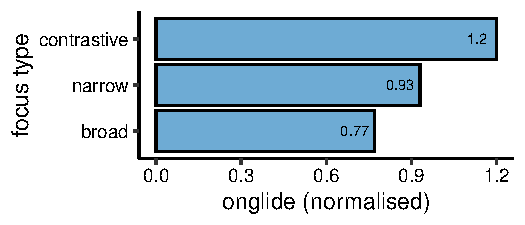
\includegraphics[width=7.5cm]{figures/ch6/onglide_norm_rising_means.pdf}
\caption{Means of rising onglides (normalised) for broad, narrow and contrastive focus.}
\label{fig:onglide_means}
\end{figure}

The results are analysed using a Bayesian linear mixed model in R \citep{RCoreTeam2018} with the package brms \citep{Buerkner2018} which implements an interface to Bayesian inference with MCMC sampling in Stan \citep{Carpenteretal2017}. The estimated differences between focus conditions in terms of posterior means are reported in addition to 95\% credible intervals, and the probability of the estimate being greater than zero. Given the data and the model, the 95\% credible intervals indicate the range in which one can be certain with a probability of 0.95 that the difference between estimates can be found. To calculate the differences between focus types,  the analysis subtracts the posterior samples for background from broad focus (broad–background), broad focus from narrow focus (narrow–broad), narrow focus from contrastive focus (contrastive–narrow), and broad focus from contrastive focus (contrastive–broad).

Normalised onglide is included as the dependent variable in the model, focus type as a fixed effect, and random intercepts for speakers and target words as well as by-speaker slopes for the effect of focus type. Since the distribution of the dependent variable is bimodal, a prior for the predictor is used that is characterised by a mixture of two Gaussian distributions centred around −0.5 and 0.5 respectively. The model estimates the parameter theta that represents the extent to which the two Gaussian distributions are mixed. This parameter is referred to as the mixing parameter. For this parameter, a prior centred around zero is used. Differences in the mixing parameter indicate differences in the proportions of the two modes in the onglide data. The model runs with four sampling chains of 3,000 iterations each.

The presentation of the results starts with the mixing parameter. Given the model and the data, the analysis yields evidence for differences in the posterior probabilities for the mixing parameter between broad focus and narrow focus ($\hat\beta=1.32, CI=[0.60, 1.95], \allowbreak Pr(\hat\beta>0)=1$), narrow focus and contrastive focus ($\hat\beta=1.59, CI=[0.56, 2.65], \allowbreak Pr(\hat\beta>0)=1$) as well as broad focus and contrastive focus ($\hat\beta=2.91, CI=[1.61, 4.09], \allowbreak Pr(\hat\beta>0)=1$).

To assess the differences between the focus conditions regarding the rising distributions, the mean estimates of the right Gaussian sub-distribution are investigated. Given the model and the data, the analysis yields evidence for differences in the posterior probabilities for the mixing parameter between broad focus and narrow focus ($\hat\beta=0.14, CI=[0.07, 0.20], \allowbreak Pr(\hat\beta>0)=1$), narrow focus and contrastive focus ($\hat\beta=0.24, CI=[0.16, 0.32], \allowbreak Pr(\hat\beta>0)=1$) as well as broad focus and contrastive focus ($\hat\beta=0.37, CI=[0.30, 0.45], \allowbreak Pr(\hat\beta>0)=1$).

\subsection{Alignment of the peak}

In addition to the scaling of an accent -- an aspect that is captured by the tonal onglide -- the alignment of the peak has been reported to be an important dimension of pitch accents \citep[see also Chapter \ref{chapter_prosody}]{Gussenhoven2004, Ladd2008, LaddMorton1997}. The measure includes not only the peak alignment of rising accents but also the peak alignment of falling accents. This means that the peaks investigated here are of two kinds in terms of an autosegmental-metrical analysis: In rising accents, H* and L+H*, the peak belongs to the starred tone, for falling accents, H+!H* or H+L*, it belongs to the leading tone.

Negative alignment values indicate that the peak is early, i.e. before the onset of the vowel, while positive alignment values characterise a mid or late peak, i.e. after the vowel onset. The latter are referred to as \emph{mid to late peaks} in what follows. Figure \ref{fig:alignment_distributions_within} presents the distributions of alignment values of all speakers together for broad, narrow and contrastive focus. Similar to the distributions of the tonal onglide, the right mode increases in relation to the left mode when going from broad to narrow focus and from narrow to contrastive focus. The numbers and proportions of early and mid to late peaks are summarised in Table \ref{tab:props_alignment}. Note that the numbers of NA data points is different from the tonal onglide as the alignment measure is only based on the time points and not on the calculation of F0 that may fail due to technical issues in some cases.

Figure \ref{fig:alignment_means}\footnote{Note that the x-axis does not start at zero.} presents the means of the positive alignments (mid to late peaks) and shows that in addition to lower proportions of early peaks, the positive alignments increase, i.e. the instances within the group of mid to late peaks become later, although the difference between narrow and contrastive focus appears to be very subtle.

\begin{figure}[p]
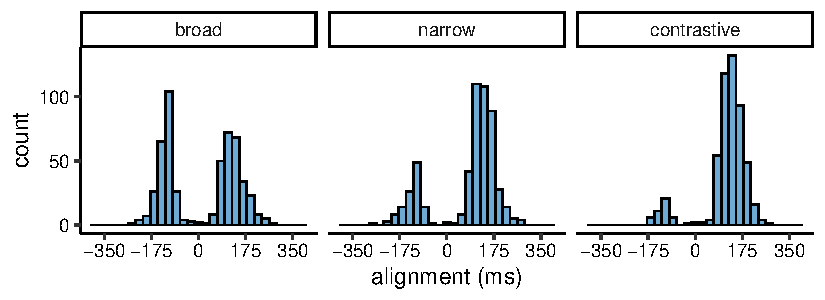
\includegraphics[width=.95\textwidth]{figures/ch6/alignment_distribution_within.pdf}
\caption{Distributions of alignment values for broad, narrow and contrastive focus.}
\label{fig:alignment_distributions_within}
\end{figure}



\begin{figure}[p]
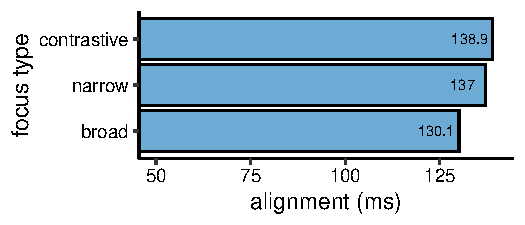
\includegraphics[width=7.5cm]{figures/ch6/alignment_mid_late_means.pdf}
\caption{Means of positive alignment values for broad, narrow and contrastive focus.}
\label{fig:alignment_means}
\end{figure}

\begin{table}[p]
	\caption{Proportions of early and mid to late alignments.}
	\begin{tabularx}{\textwidth}{Xllll}
		\lsptoprule
		\textbf{focus types	} &	\textbf{early peak}&		\textbf{mid to late peak} &		\textbf{NA} & 	\textbf{all}\\
		&				\textbf{(negative alignment)} &	\textbf{(positive alignment)} &		&			\\	
		\midrule
		broad focus &		241 (47.07\%) & 				271 (52.93\%)  & 					0 (0\%) &			512	\\
		%&				47.07\% &				52.93\% &					0\% &			\\
		%\midrule
		narrow focus &		117 (22.16\%)  &				411 (77.84\%) & 					0 (0\%)  &			528 \\
		%&				22.16\% &				77.84\% & 					0\% &			\\
		%\midrule
		contrastive focus &		47 (9.04\%)  &					473 (90.96\%) &						0 (0\%) &			520 \\
		%&				9.04\% &				90.96\% &					0\% &			\\
		\midrule
		all &				405 (25.96\%) &					1155 (74.04\%)  &					0 (0\%) &			1560	\\\lspbottomrule
		%&				25.96\% & 				74.04\% &					0\% & 		\\ \lspbottomrule
	\end{tabularx}
	\label{tab:props_alignment}
\end{table}%

A similar Bayesian model to the one employed for the tonal onglide is used. The dependent variable is changed to alignment. For the mixing parameter a bimodal prior centred around −130 and 130, respectively, is used. Everything else is parallel to the statistical modelling of tonal onglide. Again, the presentation of the results starts with the mixing parameter. Given the model and the data, the analysis yields evidence for differences in the posterior probabilities for the mixing parameter between broad focus and narrow focus ($\hat\beta=1.29 , CI=[0.56, 1.91], \allowbreak Pr(\hat\beta>0)=1$), narrow focus and contrastive focus ($\hat\beta=1.56, CI=[0.50, 2.60],\allowbreak Pr (\hat\beta>0)=0.99$) as well as broad focus and contrastive focus ($\hat\beta = 2.85, CI=[1.48, 4.10], \allowbreak Pr(\hat\beta>0)=1$).

As in the case of tonal onglide, the mean estimates of the right Gaussian sub-distribution are investigated to assess the differences between the focus conditions regarding the rising distributions. Given the model and the data, the analysis yields evidence for differences in the posterior probabilities for the mixing parameter between broad focus and contrastive focus ($\hat\beta=7.72, CI=[2.22, 13.50], \allowbreak Pr(\hat\beta>0)=1$). The evidence is weaker for differences between broad focus and narrow focus ($\hat\beta=5.86, CI=[-0.22, 11.36], \allowbreak Pr(\hat\beta>0)=0.98$) and between narrow focus and contrastive focus ($\hat\beta=1.86, CI=[-3.56, 6.74], \allowbreak Pr(\hat\beta>0)=0.75$), confirming the impression given by Figure \ref{fig:alignment_means} that the peak alignments of narrow and contrastive focus are closer compared to those of broad and contrastive focus.

\section{Modelling account}

The data presented in the last sections reveal two major results: First, distributions of pitch accent types (rising/falling, early/mid to late) are overlapping between focus types but there are clear trends for more rising and more mid to late accents in narrow compared to broad focus, and in contrastive compared to narrow focus. Second, more subtle modifications in the positive portions of both distributions (i.e. rising accents and mid to late accents) take place as well. The magnitudes of the rising onglides increase and the mid to late peaks are aligned later. These findings point towards an intertwining of categorical and continuous aspects of prosodic focus marking. It could be described as a case of a parallel between the phonetics and the phonology of intonation in which one ``mimics" the other.

This interpretation motivates a modelling approach that describes both categorical and continuous aspects in the same formal system. Chapter \ref{chapter_ds} discussed the role of dynamical systems for such a modelling approach. The current section applies a dynamical model to the description of the pitch accent data outlined above for the dimension of tonal onglide. The alignment of the peak exhibits comparable results to those of the tonal onglide and, hence, the outlined model for tonal onglide will in general be applicable to this parameter as well. Since the distributions of tonal onglide show bimodal patterns, it seems natural to employ a system with two attractors as the one given by the potential $V(x)$ and the force $F(x)$ in Equation \ref{eq:onglide_model}. 

This dynamical system is similar to the systems with double-well potentials discussed extensively in Chapter \ref{chapter_ds}. The reader is reminded that the scaling of the control parameter in these systems (e.g. $k$ in Equation \ref{eq:onglide_model}) tilts the potential, the attractor landscape, to one side or the other, lending more stability to one of the attractors. In a stochastic conception of the system, it is more likely that the system settles in the more stable attractor as more noise is needed to push the system out of the ``deeper", more stable attractor. When the control parameter is zero, both attractors are equally stable. For all other values, one attractor is more stable than the other. Past critical thresholds of the control parameter on both sides (negative and positive), the system bifurcates and only one attractor remains. 
\begin{equation}
\begin{split}
V(x) = -kx + \frac{x^4}{4} - x^2 \\
F(x) = k - x^3 + 2x
\label{eq:onglide_model}
\end{split}
\end{equation}

The emphasis of the approach outlined here is on the qualitative correspondence of the experimental observations and the theoretical model. The coefficients for the model are chosen for presentation purposes, the system does not produce the same scale as the real data. As will become clear in the course of the section, the presented system is able to capture at least the most important aspects of the structure of the data. The choice of two attractors, as stated above, is motivated by the structure of the data. Using a system with two attractors for the model does not imply that there are only two pitch accent categories in German. The GToBI model of German intonation \citep{GriceBaumann2002} posits six distinct accent types, although the importance of the differentiation between H+L* and H+!H* has decreased as there is only little evidence for a difference between the two. It is thus not uncommon to treat falling accents as one group. Furthermore, the current data set does not exhibit instances of L* accent types (L*+H and L*). 

As to the differentiation between the rising pitch accent types H* and L+H*, it can be stated that neither the positive portion of the alignment data, nor the positive portion of the tonal onglide data reveal a bimodal shape. Assuming only a single rising accent type is thus data-driven and does not claim that the intonational system of German is structured this way.

The control parameter $k$ which occurs in the functions of Equation \ref{eq:onglide_model} is used to modulate the attractor landscape such that one attractor becomes more stable and hence more resistant to noise. The attractor landscape is symmetrical with $k=0$. For broad focus, a value of $k$ slightly above $0$ can be used, e.g. $k=0.1$, tilting the landscape subtly to the right while retaining the characteristics of two nearly symmetrical attractors. For narrow focus, the value of the control parameter $k$ has to increase such that the right attractor, the ``rising attractor", becomes more stable. In the present model, $k$ is set to $0.45$ in narrow focus. For contrastive focus, the system has to tilt even more to the right side. Hence, a higher number, $k=0.9$, is chosen. Figure \ref{fig:potentials_force_br_na_co} plots the graphs of the resulting potential and force functions with this parametrisation of $k$.

\begin{figure}
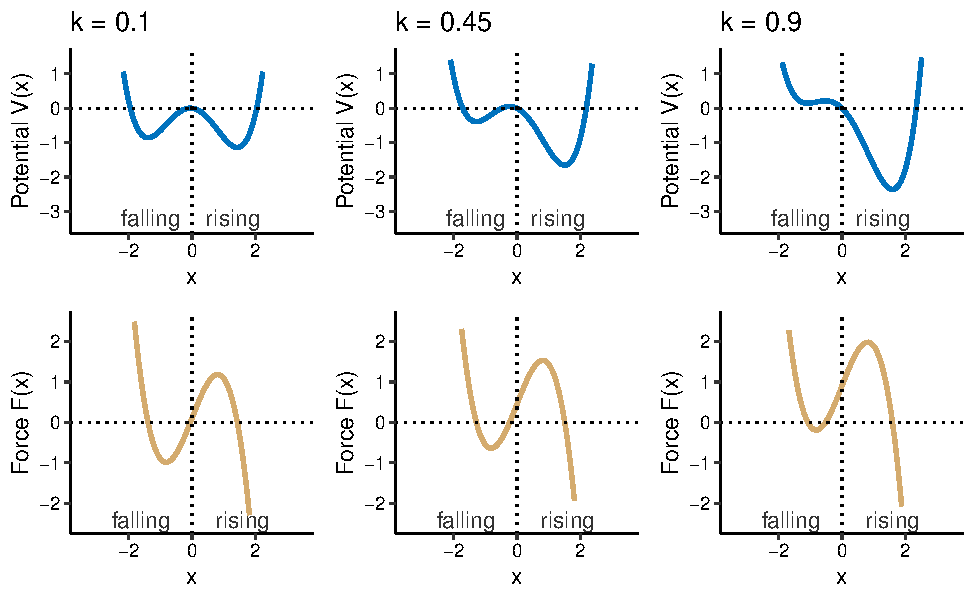
\includegraphics[width=\textwidth]{figures/ch6/potentials_force.pdf}
\caption{Potential and force functions for $k$ values modelling broad, narrow and contrastive focus.}
\label{fig:potentials_force_br_na_co}
\end{figure}

Simulations are run on these attractor landscapes. The methodology of the simulation is as described in Chapter \ref{chapter_ds}: The system is conceptualised as a stochastic system that exhibits random fluctuations. The differential function describing the system (the force function) is solved using small discrete time steps. Noise is added in each of these time steps. The noise in this case is a random number from a Gaussian distribution with a mean of $0$ and standard deviation of $0.03$. The simulation is finished after 5,000 time steps and records the solution. This procedure is repeated to obtain 2,500 solutions for each value of $k$.

Figure \ref{fig:simulation_br_na_co} presents the results of one simulation for each of the $k$ values chosen to model the focus types (broad: $0.1$, narrow: $0.45$, contrastive: $0.9$). The histograms show the characteristic pattern of the real tonal onglide data (see Figure \ref{fig:onglide_distributions_within} for comparison): almost equal numbers of rises and falls in broad focus and increasing numbers of rises in narrow and contrastive focus. In Figure \ref{fig:simulation_means_br_na_co}, the means of the positive sub-distributions of the stimulation results are displayed. This figure also indicates a strong correspondance of the simulated data to the real data (compare to Figure \ref{fig:onglide_means}).  It becomes evident that while making the right (rising) attractor more stable, the attractor basin also shifts subtly towards more extreme values in the state space. This accounts for the observed pattern of increasing onglide magnitudes from broad to narrow focus and narrow to contrastive focus in the data. The phenomenon can be observed in Figure \ref{fig:right_basin}. This graph displays the right attractor basin for broad focus, narrow focus and contrastive focus, i.e. $k=0.1$, $k=0.45$ and $k=0.9$, plotted on top of each other. The vertical lines (solid for $k=0.1$, dotted for $k=0.45$, dashed for $k=0.9$)  indicate the location of the attractor that moves to the right, i.e. larger values for rising onglides with the increase in $k$.

\begin{figure}
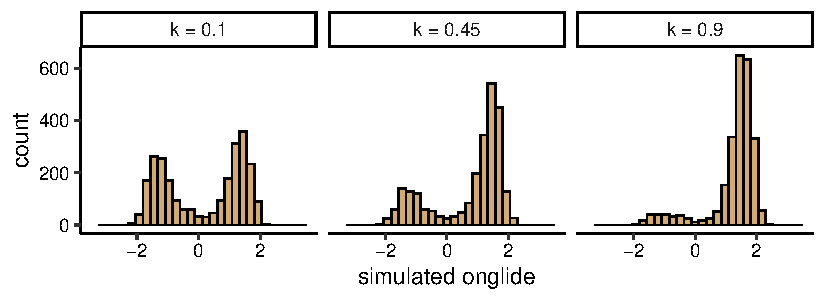
\includegraphics[width=\textwidth]{figures/ch6/onglide_all_within.pdf}
\caption[Distributions of simulation results for $k$ values modelling broad ($k=0.1$), narrow ($k=0.45$) and contrastive focus ($k=0.9$).]{Distributions of simulation results for $k$ values modelling broad, narrow and contrastive focus (from left to right).}
\label{fig:simulation_br_na_co}
\end{figure}

\begin{figure}
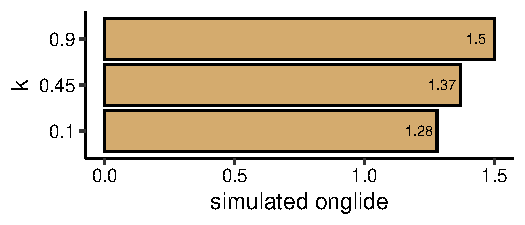
\includegraphics[width=7.5cm]{figures/ch6/positive_means_within.pdf}
\caption{Means of positive simulated onglides for $k$ values modelling broad ($k=0.1$), narrow ($k=0.45$) and contrastive focus ($k=0.9$).}
\label{fig:simulation_means_br_na_co}
\end{figure}

\begin{figure}
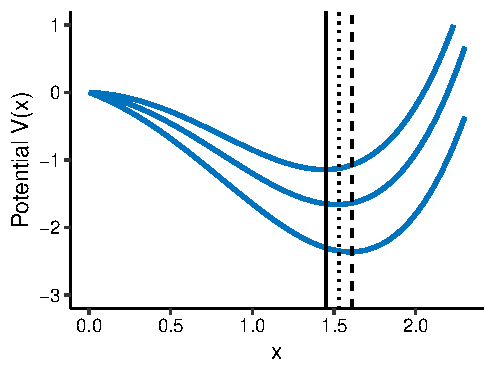
\includegraphics[width=7.5cm]{figures/ch6/right_basin.pdf}
\caption[Zoom of right (rising) attractor basin.]{Zoom of right (rising) attractor basin. The vertical lines mark the location of the attractor. Solid line: broad focus; dotted line: narrow focus; dashed line: contrastive focus.}
\label{fig:right_basin}
\end{figure}

The modelling account outlined here employs a rather simple dynamical mod\-el that posits two attractor in a continuous state space. This state space is made up of only one dimension, namely the tonal onglide. Of course, this is a simplification: Pitch accents are best seen as multi-dimensional, as the alignment measure for instance demonstrated. A full model would include all relevant parameters. However, reducing the model to one dimension makes it more transparent. The present model is best seen as a proof of concept that is able to capture important generalisations in the data about the interplay of categorical and continuous aspects of intonation. The centrepiece of the model is the idea that phonological categories are not separated from their phonetic implementation. The stability relations, i.e. the presence of an attractor, position the categories (falling / rising accents) in the continuum of the state space. The phonetic realisation (magnitude of the movement in terms of onglide) follows from this position on the continuum. The category and the phonetic realisation are thus deeply intertwined and inseparable.

\section{Speaker groups}

With the dynamical model for pitch accents sketched, the question arises as to whether all speakers use the system in the same way. Even with as few subjects as five, \citet{Griceetal2017} could observe different strategies: One group of speakers used qualitative modifications, i.e. different pitch accent types, to differentiate between focus types, the other group used rising pitch accents only but produced more subtle quantitative variation in the realisation of the pitch accents. To assess these differences in the present data set, speakers were grouped according to their overall pattern of pitch accent productions. Group 1 consists of the 11 speakers who use falling onglides in more than 33\% of the cases overall. Group 2 consists of the 16 speakers who use up to 33\% falling onglides overall. Group 1 thus pools the speakers that make frequent use of clearly qualitatively different tonal onglide patterns, while the speakers in group 2 only rarely make use of a falling-rising distinction. 

The distributions of tonal onglide values for the two groups are given in Figure \ref{fig:onglide_distributions_groups}. For group 1, the distributions of broad, narrow and contrastive focus are more distinct. In broad focus, falling accents are most frequent; in narrow focus the distribution is dominated by rising accents but there is a considerable number of falling accents; in contrastive focus there is only a small number of falling accents. For group 2, the distributions appear less distinct. Rising onglides are predominantly used in all three focus types, although there is a small number of falling accents in broad focus and an even smaller number of falling accents in narrow focus. Hence, a minimal version of the trend observed for group 1, and the group of all speakers, can be attested here as well, i.e. less falls and more rises from broad to narrow focus and from narrow to contrastive focus.

\begin{figure}[t]
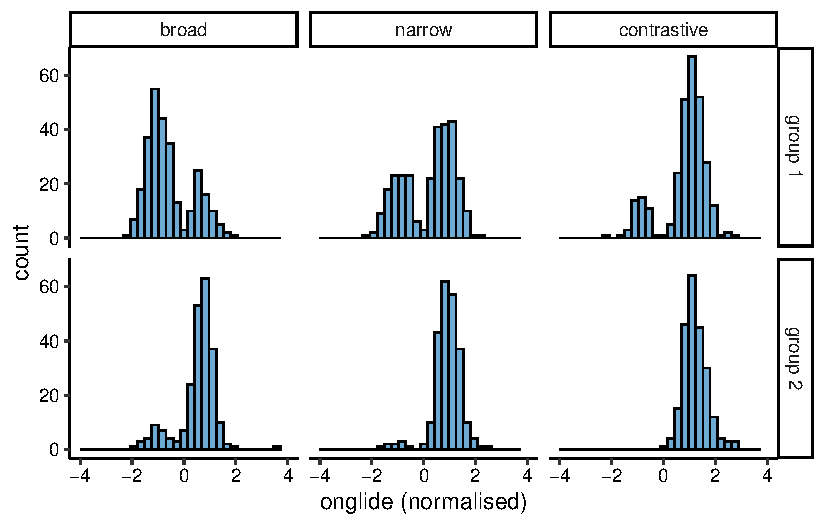
\includegraphics[width=\textwidth]{figures/ch6/onglide_norm_distribution_within_groups.pdf}
\caption[Distributions of normalised tonal onglide values for broad, narrow and contrastive focus, separately for the two speaker groups.]{Distributions of normalised tonal onglide values for broad, narrow and contrastive focus, separately for the two speaker groups. Top: group 1, bottom: group 2.}
\label{fig:onglide_distributions_groups}
\end{figure}

Figure \ref{fig:onglide_means_group1} and Figure \ref{fig:onglide_means_group2} display the means of the rising onglide distributions for the two speaker groups. For both groups, the means increase when going from broad through narrow to contrastive focus, indicating that the magnitudes of rising onglides become larger. In addition to this main trend, the means of group 2 are slightly higher overall than those of group 1.

\begin{figure}
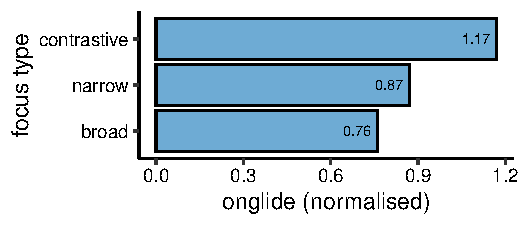
\includegraphics[width=7.5cm]{figures/ch6/onglide_norm_rising_means_group1.pdf}
\caption{Means of rising onglides (normalised) of speaker group 1 for broad, narrow and contrastive focus.}
\label{fig:onglide_means_group1}
\end{figure}

\begin{figure}
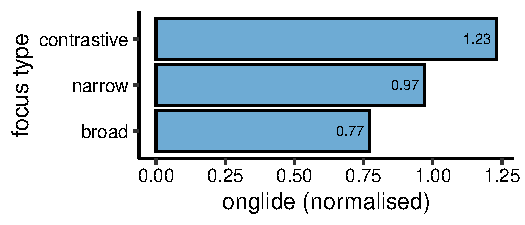
\includegraphics[width=7.5cm]{figures/ch6/onglide_norm_rising_means_group2.pdf}
\caption{Means of rising onglides (normalised) of speaker group 2 for broad, narrow and contrastive focus.}
\label{fig:onglide_means_group2}
\end{figure}

In terms of the dynamical model outlined above, the behaviour of the speaker groups can be captured by choosing different values for the control parameter $k$. For group 1, broad focus may be modelled with $k = -0.4$, narrow focus with $k = 0.3$, and contrastive focus with $k = 0.8$. For group 2, broad focus may be modelled with $k = 0.8$, narrow focus with $k =  1.0$, and contrastive focus with $k = 1.2$. Crucially, in all cases, the scaling of the control parameter goes in the same direction: broad focus < narrow focus < contrastive focus. The resulting attractor landscapes are plotted in Figure \ref{fig:potentials_groups} for group 1 (top) and group 2 (bottom), the $k$ values chosen for the groups are compared graphically in Figure \ref{fig:groups_k}. In all cases, the model predicts less falling onglides from broad to narrow focus and from narrow to contrastive focus. The initial proportion of falling and rising accents differs between the group, the direction or mechanism of modification is comparable. In addition, the model predicts increasing magnitudes of the rising onglides and a higher overall level of rises in group 2 compared to group 1. It should be noted that the latter prediction -- the overall higher level of rising onglides in group 2 -- poses a limitation in the correspondence between the model and the real data. As a comparison of Figure \ref{fig:onglide_means_group1} and Figure \ref{fig:onglide_means_group2} shows, the means of the rises are higher in group 2, and thus the pattern predicted by the model can be found in the data. The difference between the two groups with regard to the means of the rises is, however, certainly less pronounced than the model predicts it.

\begin{figure}[t]
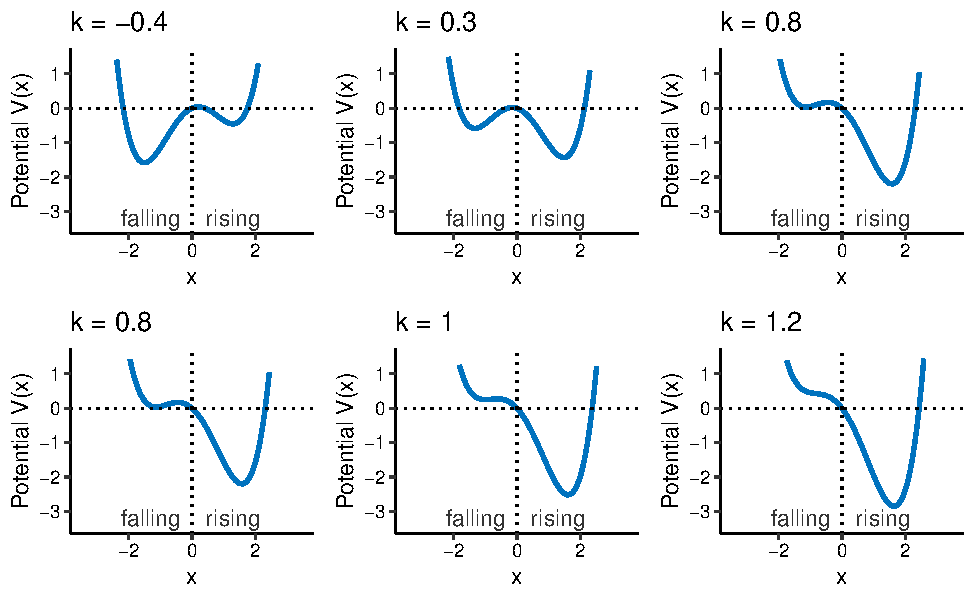
\includegraphics[width=\textwidth]{figures/ch6/potentials_groups.pdf}
\caption[Potential and force functions for $k$ values modelling broad (left), narrow (centre) and contrastive focus (right), separately for the two speaker groups.]{Potential and force functions for $k$ values modelling broad, narrow and contrastive focus, separately for the two speaker groups. Top: group 1, bottom: group 2.}
\label{fig:potentials_groups}
\end{figure}

\begin{figure}
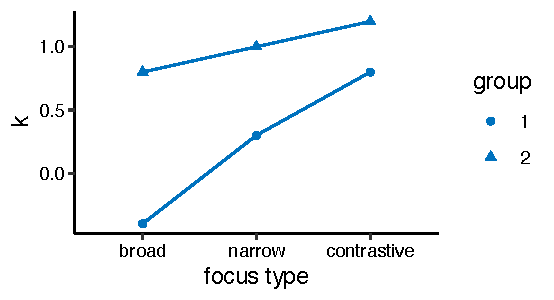
\includegraphics[width=8.5cm]{figures/ch6/groups_k.pdf}
\caption{Control parameter values $k$ of the two speaker groups.}
\label{fig:groups_k}
\end{figure}

The discussion of these differences between speakers raises the question as to how communication is possible if the speakers' behaviour is so different. Since the current analysis includes only production results, no direct evidence for the effect on perception can be provided here. However, three points appear important to note. First, as pointed out in Chapter \ref{chapter_prosody}, the perception results of \citet{CangemiKrügerGrice2015} -- in which listeners rated the productions analysed in \citet{Griceetal2017} and \citet{MückeGrice2014} -- provide evidence that both speaker types yield comparable scores overall in perception. Some listeners preferred the categorical speakers (comparable to group 1) while other listeners preferred the more subtle speakers (comparable to group 2). Second, it has to be emphasised that tonal onglide only represents one of many dimensions in which pitch accents can vary, or as \citet[143]{CangemiKrügerGrice2015} put it: ``Rather than singly necessary and jointly sufficient features for category membership, phonetic cues are better understood as dimensions along which phonological categories cluster, in an individual-specific network of phonological knowledge". Third, in the light of evidence for phonetic accommodation \citep[e.g.][]{YuAbregoCollierSonderegger2013, Babel2009}, it may be plausible to assume that listeners are able to ``tune in" to a speaker and adjust their perceptual patterns to the production patterns of the speaker. Listeners may be able to quickly learn (or recall) the prosodic patterns of their interlocutor and adjust their mappings of forms and functions.

\section{Summary}

This section provided an analysis of nuclear pitch accents used to mark focus structure in German by 27 native speakers. The parameters investigated were tonal onglide and alignment of the peak. The analysis showed that speakers use categorical as well as continuous modifications to express different focus structures. Crucially, both types of modification appear to go hand in hand. From broad to narrow, and from narrow to contrastive focus, more rising and more mid to late peak accents (and less falling and early peak accents) are found. In addition, the magnitude of the tonal onglide of the rises and the peak alignment of the mid to late accents increase at the same time. These results support a perspective that emphasises an intertwining of categorical and continuous aspects of prosody and call for an integration of the two in a theoretical treatment. A dynamical model was proposed that does not separate phonological categories from their phonetic implementation and thus provides a first step towards treating both types of modifications as the outcome of the same system. Furthermore, it was shown that speakers differ in how they use the system while maintaining the general direction of scaling of the control parameter.

